\documentclass[a4paper,10pt]{article}
\usepackage[utf8]{inputenc}
\usepackage[T1]{fontenc}
\usepackage[provide=*,french]{babel}
\usepackage{lmodern}
\usepackage[left=0.72cm,right=0.72cm,top=0.48cm,bottom=0.78cm]{geometry}
\usepackage{tikz}
\usepackage{graphicx}
\usepackage{xcolor}
\usepackage{eso-pic}
\usepackage{amsmath,amssymb}
\usetikzlibrary{calc,arrows.meta,positioning}

\pagestyle{empty}
\renewcommand{\familydefault}{\sfdefault}
\setlength{\parindent}{0pt}
\renewcommand{\arraystretch}{1.15}

\definecolor{brandNavy}{RGB}{11,53,112}
\definecolor{brandBlue}{RGB}{17,70,140}
\definecolor{brandTeal}{RGB}{29,174,174}
\definecolor{brandOrange}{RGB}{255,145,20}
\definecolor{softBlue}{RGB}{225,238,255}
\definecolor{softTeal}{RGB}{219,247,246}
\definecolor{softOrange}{RGB}{255,238,215}
\definecolor{softGray}{RGB}{245,247,250}

\newcommand{\LogoFile}{../assets/img/mathsgo-logo.png}
\newcommand{\MathsGoFooter}{%
\begin{tikzpicture}[remember picture,overlay]
  \node[anchor=south west,inner sep=0pt] at ([xshift=0.55cm,yshift=0.18cm]current page.south west)
    {\includegraphics[width=2.45cm]{\LogoFile}};
  \node[anchor=south,inner sep=0pt,text=brandNavy!70,font=\sffamily\bfseries\fontsize{7}{7}\selectfont]
    at ([yshift=0.32cm]current page.south) {mathsgo.re};
\end{tikzpicture}%
}
\AddToShipoutPictureFG{\MathsGoFooter}

\newcommand{\Badge}[1]{\tikz[baseline=-0.62ex]{\node[circle,fill=brandNavy,text=white,font=\bfseries,minimum size=0.50cm,inner sep=0pt]{#1};}}
\newcommand{\Section}[2]{\Badge{#1}\hspace{0.15cm}{\bfseries\color{brandNavy}\fontsize{11.7}{12.4}\selectfont #2}}
\newcommand{\LowDotted}[1]{%
\begin{tikzpicture}[baseline=-0.78ex]
  \draw[densely dotted,line width=0.70pt,line cap=round] (0,-0.22) -- (#1,-0.22);
\end{tikzpicture}}
\newcommand{\CheckBox}{\ensuremath{\Box}\,}
\newcommand{\BigRatio}[1]{{\fontsize{15.0}{16.0}\selectfont\displaystyle #1}}
\newcommand{\Apt}{\textcolor{brandOrange}{A}}
\newcommand{\Mpt}{\textcolor{brandBlue}{M}}
\newcommand{\Npt}{\textcolor{brandBlue}{N}}
\newcommand{\Bpt}{\textcolor{brandTeal}{B}}
\newcommand{\Cpt}{\textcolor{brandTeal}{C}}
\newcommand{\AMcol}{\textcolor{brandOrange}{A}\textcolor{brandBlue}{M}}
\newcommand{\ANcol}{\textcolor{brandOrange}{A}\textcolor{brandBlue}{N}}
\newcommand{\ABcol}{\textcolor{brandOrange}{A}\textcolor{brandTeal}{B}}
\newcommand{\ACcol}{\textcolor{brandOrange}{A}\textcolor{brandTeal}{C}}
\newcommand{\MNcol}{\textcolor{brandBlue}{M}\textcolor{brandBlue}{N}}
\newcommand{\BCcol}{\textcolor{brandTeal}{B}\textcolor{brandTeal}{C}}

\newcommand{\FigureEmboitee}[1]{%
\begin{tikzpicture}[scale=#1,line cap=butt,line join=miter]
  \coordinate (A) at (0,0);
  \coordinate (B) at (5.40,-1.20);
  \coordinate (C) at (4.70,2.20);
  \coordinate (M) at (2.59,-0.58);
  \coordinate (N) at (2.26,1.06);
  \fill[softTeal!38] (A)--(B)--(C)--cycle;
  \draw[brandNavy,line width=1.20pt] (A)--(M);
  \draw[brandNavy,line width=1.20pt] (A)--(N);
  \draw[brandNavy,line width=1.24pt] (M)--(N);
  \draw[brandBlue,line width=1.20pt] (M)--(B);
  \draw[brandBlue,line width=1.20pt] (N)--(C);
  \draw[brandTeal,line width=1.34pt] (B)--(C);
  \node[brandOrange,font=\bfseries\small] at (-0.27,-0.25) {$A$};
  \node[brandBlue,font=\bfseries\small] at (2.62,-0.88) {$M$};
  \node[brandBlue,font=\bfseries\small] at (2.04,1.28) {$N$};
  \node[brandTeal,font=\bfseries\small] at (5.68,-1.18) {$B$};
  \node[brandTeal,font=\bfseries\small] at (4.89,2.42) {$C$};
\end{tikzpicture}}

\newcommand{\FigurePapillon}[1]{%
\begin{tikzpicture}[scale=#1,line cap=butt,line join=miter]
  \coordinate (A) at (0,0);
  \coordinate (B) at (3.40,-1.20);
  \coordinate (C) at (2.60,1.90);
  \coordinate (M) at (-2.21,0.78);
  \coordinate (N) at (-1.69,-1.24);
  \draw[brandNavy,line width=1.20pt] (M)--(A);
  \draw[brandNavy,line width=1.20pt] (N)--(A);
  \draw[brandNavy,line width=1.24pt] (M)--(N);
  \draw[brandTeal,line width=1.20pt] (A)--(B);
  \draw[brandTeal,line width=1.20pt] (A)--(C);
  \draw[brandTeal,line width=1.34pt] (B)--(C);
  \node[brandOrange,font=\bfseries\small] at (-0.05,0.31) {$A$};
  \node[brandBlue,font=\bfseries\small] at (-2.50,0.94) {$M$};
  \node[brandBlue,font=\bfseries\small] at (-1.93,-1.43) {$N$};
  \node[brandTeal,font=\bfseries\small] at (3.68,-1.21) {$B$};
  \node[brandTeal,font=\bfseries\small] at (2.80,2.12) {$C$};
\end{tikzpicture}}

\newcommand{\BlankEmboitee}[1]{%
\begin{tikzpicture}[scale=#1,line cap=butt,line join=miter]
  \coordinate (A) at (0,0);
  \coordinate (B) at (5.40,-1.20);
  \coordinate (C) at (4.70,2.20);
  \coordinate (M) at (2.59,-0.58);
  \coordinate (N) at (2.26,1.06);
  \fill[softTeal!22] (A)--(B)--(C)--cycle;
  \draw[brandNavy!90,line width=1.10pt] (A)--(M);
  \draw[brandNavy!90,line width=1.10pt] (A)--(N);
  \draw[brandNavy!90,line width=1.15pt] (M)--(N);
  \draw[brandBlue,line width=1.10pt] (M)--(B);
  \draw[brandBlue,line width=1.10pt] (N)--(C);
  \draw[brandTeal,line width=1.18pt] (B)--(C);
  \node at (-0.55,-0.45) {\LowDotted{0.48}};
  \node at (2.82,-1.08) {\LowDotted{0.48}};
  \node at (1.82,1.50) {\LowDotted{0.48}};
  \node at (6.02,-1.35) {\LowDotted{0.48}};
  \node at (4.90,2.68) {\LowDotted{0.48}};
\end{tikzpicture}}

\newcommand{\BlankPapillon}[1]{%
\begin{tikzpicture}[scale=#1,line cap=butt,line join=miter]
  \coordinate (A) at (0,0);
  \coordinate (B) at (3.40,-1.20);
  \coordinate (C) at (2.60,1.90);
  \coordinate (M) at (-2.21,0.78);
  \coordinate (N) at (-1.69,-1.24);
  \draw[brandNavy!90,line width=1.10pt] (M)--(A);
  \draw[brandNavy!90,line width=1.10pt] (N)--(A);
  \draw[brandNavy!90,line width=1.15pt] (M)--(N);
  \draw[brandTeal,line width=1.10pt] (A)--(B);
  \draw[brandTeal,line width=1.10pt] (A)--(C);
  \draw[brandTeal,line width=1.18pt] (B)--(C);
  \node at (0.00,0.55) {\LowDotted{0.48}};
  \node at (-2.72,1.20) {\LowDotted{0.48}};
  \node at (-2.05,-1.68) {\LowDotted{0.48}};
  \node at (4.00,-1.40) {\LowDotted{0.48}};
  \node at (2.95,2.38) {\LowDotted{0.48}};
\end{tikzpicture}}

\begin{document}

% ================= PAGE 1 : COMPRENDRE =================
\begin{center}
{\fontsize{21.0}{22.0}\selectfont\bfseries\color{brandNavy} Théorème de Thalès : calculer une longueur}\par\vspace{0.02cm}
{\fontsize{12.4}{13.1}\selectfont\bfseries\color{brandTeal} La version directe}
\end{center}

\vspace{0.02cm}
\begin{center}
\begin{minipage}[t]{9.15cm}
\centering
\tikz\node[rounded corners=7pt,draw=brandTeal!65,fill=brandTeal!3,line width=0.70pt,text width=8.70cm,inner sep=5pt,align=center]{%
{\bfseries\color{brandTeal} Cas emboîté}\par\vspace{-0.02cm}
\FigureEmboitee{0.62}\par\vspace{-0.03cm}
{\small $\Apt-\Mpt-\Bpt$ \qquad et \qquad $\Apt-\Npt-\Cpt$}
};
\end{minipage}\hfill
\begin{minipage}[t]{9.15cm}
\centering
\tikz\node[rounded corners=7pt,draw=brandOrange!70,fill=softOrange!25,line width=0.70pt,text width=8.70cm,inner sep=5pt,align=center]{%
{\bfseries\color{brandOrange} Cas papillon}\par\vspace{-0.02cm}
\FigurePapillon{0.66}\par\vspace{-0.03cm}
{\small $\Mpt-\Apt-\Bpt$ \qquad et \qquad $\Npt-\Apt-\Cpt$}
};
\end{minipage}
\end{center}

\vspace{0.34cm}
\Section{1}{Je vérifie que je peux utiliser le théorème de Thalès}\par\vspace{0.04cm}
\begin{center}
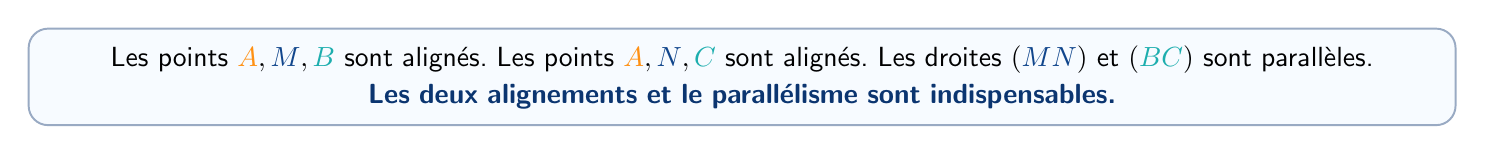
\begin{tikzpicture}
\node[rounded corners=7pt,draw=brandNavy!42,fill=softBlue!26,line width=.70pt,text width=17.70cm,inner sep=6pt,align=center] {
{\fontsize{9.6}{10.3}\selectfont Les points $\Apt,\Mpt,\Bpt$ sont alignés. Les points $\Apt,\Npt,\Cpt$ sont alignés. Les droites $(\MNcol)$ et $(\BCcol)$ sont parallèles.}\par\vspace{0.05cm}
{\bfseries\color{brandNavy} Les deux alignements et le parallélisme sont indispensables.}
};
\end{tikzpicture}
\end{center}

\vspace{0.38cm}
\Section{2}{Je construis le tableau de proportionnalité}\par\vspace{0.11cm}
\begin{center}

\begin{tikzpicture}
\node[rounded corners=8pt,draw=brandTeal!70,fill=softTeal!30,line width=.75pt,text width=17.75cm,inner sep=10pt,align=center] {
{\fontsize{10.0}{10.7}\selectfont\bfseries\color{brandNavy} Dans une même colonne, les deux longueurs se correspondent.}\par\vspace{0.18cm}
{\renewcommand{\arraystretch}{1.58}\fontsize{10.7}{11.4}\selectfont
$\displaystyle
\begin{array}{|c|c|c|c|}\hline
\substack{\text{Petit triangle }\Apt\Mpt\Npt\\\text{(en cm)}} & \AMcol & \ANcol & \MNcol\\ \hline
\substack{\text{Grand triangle }\Apt\Bpt\Cpt\\\text{(en cm)}} & \ABcol & \ACcol & \BCcol\\ \hline
\end{array}$}\par\vspace{0.22cm}
{\fontsize{15.5}{16.5}\selectfont
$\displaystyle \frac{\AMcol}{\ABcol}\mkern-8mu=\mkern-8mu\frac{\ANcol}{\ACcol}\mkern-8mu=\mkern-8mu\frac{\MNcol}{\BCcol}$}
};
\end{tikzpicture}
\end{center}

\vspace{0.42cm}
\Section{3}{Je garde les deux colonnes utiles}\par\vspace{0.10cm}
\begin{center}{\fontsize{9.4}{10.1}\selectfont\bfseries\color{brandNavy} Je garde la colonne qui contient la longueur cherchée et une colonne entièrement connue.}\end{center}\vspace{0.14cm}
\begin{center}

\begin{tikzpicture}
\node[rounded corners=7pt,draw=brandBlue!65,fill=softBlue!35,line width=.70pt,text width=7.25cm,minimum height=1.48cm,inner sep=7pt,align=center] (unknown) at (-4.45,0) {
{\bfseries\color{brandBlue} La colonne avec l'inconnue}\par\vspace{0.04cm}
{\fontsize{9.0}{9.7}\selectfont Elle contient la longueur que je cherche.}
};
\node[font=\bfseries\color{brandNavy}\fontsize{17}{18}\selectfont] at (0,0) {$=$};
\node[rounded corners=7pt,draw=brandTeal!65,fill=softTeal!35,line width=.70pt,text width=7.25cm,minimum height=1.48cm,inner sep=7pt,align=center] (known) at (4.45,0) {
{\bfseries\color{brandTeal} Une colonne complète}\par\vspace{0.04cm}
{\fontsize{9.0}{9.7}\selectfont Ses deux longueurs sont connues.}
};
\end{tikzpicture}
\end{center}
\vspace{0.12cm}
\begin{center}
\tikz\node[rounded corners=6pt,draw=brandOrange!55,fill=softOrange!32,line width=.65pt,text width=16.8cm,inner sep=5.5pt,align=center]{%
{\bfseries\color{brandOrange}\fontsize{9.2}{9.9}\selectfont Exemple : je cherche $AC$}\par\vspace{0.06cm}
$\displaystyle \frac{\ANcol}{\ACcol}=\frac{\AMcol}{\ABcol}$
\hspace{0.55cm}{\bfseries\color{brandNavy} ou}\hspace{0.55cm}
$\displaystyle \frac{\ANcol}{\ACcol}=\frac{\MNcol}{\BCcol}$\par\vspace{0.05cm}
{\fontsize{8.7}{9.4}\selectfont Je choisis l'égalité dont l'autre colonne est complète.}};
\end{center}

\vspace{0.46cm}
\Section{4}{Le modèle de rédaction}\par\vspace{0.10cm}
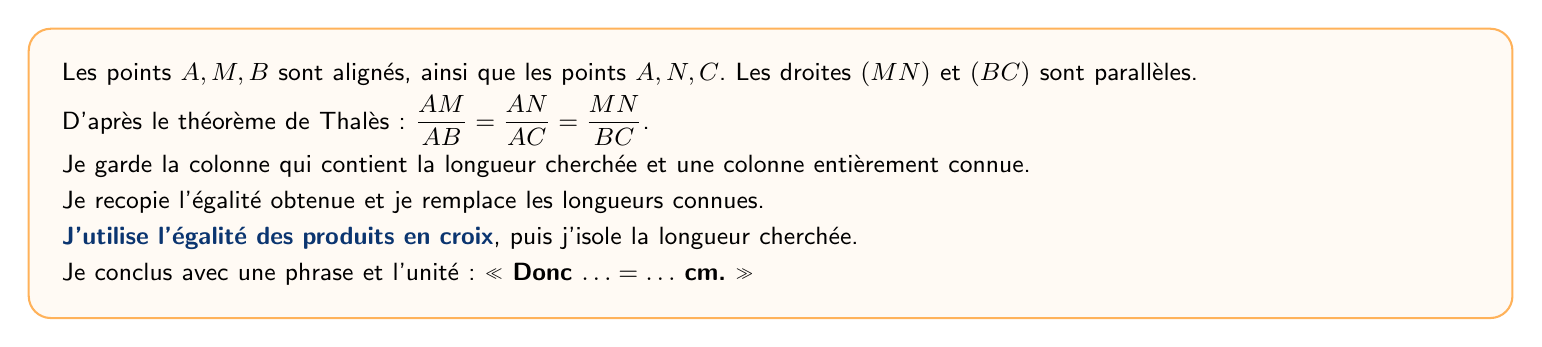
\begin{tikzpicture}
\node[rounded corners=8pt,draw=brandOrange!70,fill=softOrange!28,line width=.75pt,text width=18.00cm,inner sep=12pt,align=left] {
\begin{minipage}{17.45cm}\fontsize{9.5}{10.7}\selectfont
Les points $A,M,B$ sont alignés, ainsi que les points $A,N,C$. Les droites $(MN)$ et $(BC)$ sont parallèles.\par\vspace{0.08cm}
D'après le théorème de Thalès : $\displaystyle \frac{AM}{AB}=\frac{AN}{AC}=\frac{MN}{BC}$.\par\vspace{0.08cm}
Je garde la colonne qui contient la longueur cherchée et une colonne entièrement connue.\par\vspace{0.08cm}
Je recopie l'égalité obtenue et je remplace les longueurs connues.\par\vspace{0.08cm}
\textbf{\textcolor{brandNavy}{J'utilise l'égalité des produits en croix}}, puis j'isole la longueur cherchée.\par\vspace{0.08cm}
Je conclus avec une phrase et l'unité : \textbf{« Donc $\ldots=\ldots$ cm. »}
\end{minipage}
};
\end{tikzpicture}

\newpage

% ================= PAGE 2 : GABARIT =================
\begin{center}
{\fontsize{20.0}{21.0}\selectfont\bfseries\color{brandNavy} Fiche-guide : calculer une longueur avec Thalès}\par\vspace{0.02cm}
{\fontsize{11.8}{12.5}\selectfont\bfseries\color{brandTeal} J'adapte les lettres à la figure de mon exercice}
\end{center}

\vspace{0.10cm}
\noindent
\begin{minipage}[t]{5.20cm}
\vspace{0pt}
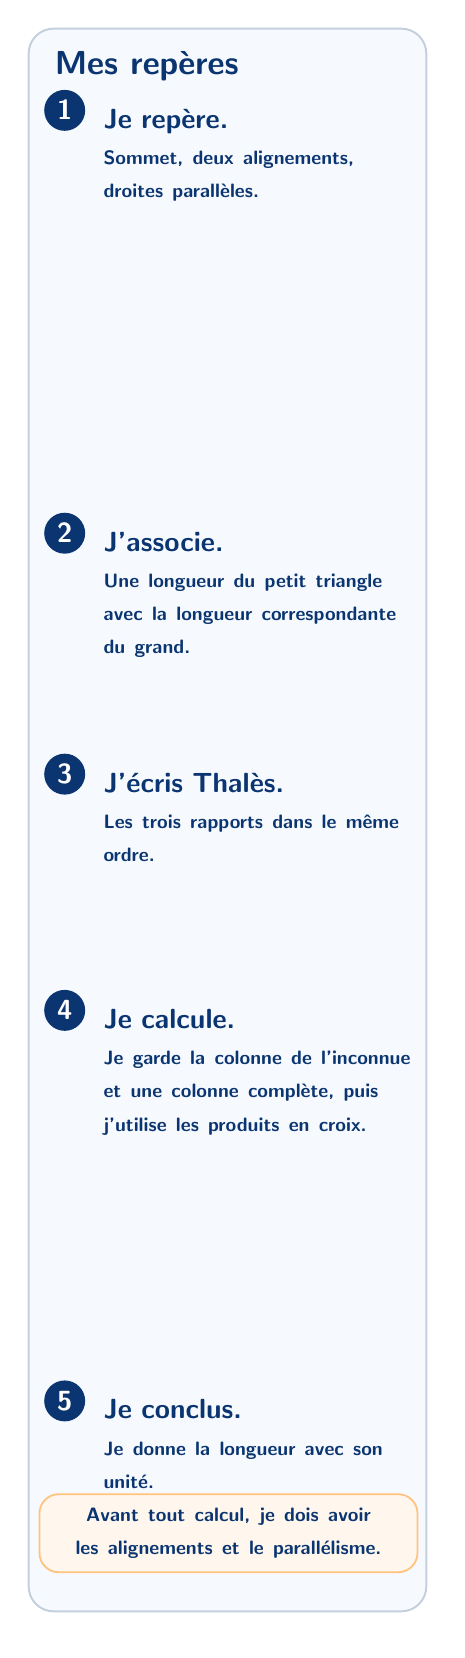
\begin{tikzpicture}[x=1cm,y=1cm]
\path[use as bounding box] (0,0) rectangle (5.20,-20.35);
\node[rounded corners=9pt,draw=brandNavy!24,fill=softBlue!30,line width=0.70pt,minimum width=5.05cm,minimum height=20.10cm,anchor=north west] at (0,0) {};
\node[anchor=north west,text=brandNavy,font=\bfseries\fontsize{12.0}{12.8}\selectfont] at (0.22,-0.18) {Mes repères};

\node[circle,fill=brandNavy,text=white,font=\bfseries,minimum size=0.52cm,inner sep=0pt] at (0.47,-1.05) {1};
\node[anchor=north west,text width=3.92cm,align=left] at (0.84,-0.91) {\bfseries\color{brandNavy}\fontsize{10.2}{10.9}\selectfont Je repère.\par\vspace{0.04cm}{\scriptsize\bfseries\color{brandNavy} Sommet, deux alignements, droites parallèles.}};

\node[circle,fill=brandNavy,text=white,font=\bfseries,minimum size=0.52cm,inner sep=0pt] at (0.47,-6.42) {2};
\node[anchor=north west,text width=3.92cm,align=left] at (0.84,-6.28) {\bfseries\color{brandNavy}\fontsize{10.2}{10.9}\selectfont J'associe.\par\vspace{0.04cm}{\scriptsize\bfseries\color{brandNavy} Une longueur du petit triangle avec la longueur correspondante du grand.}};

\node[circle,fill=brandNavy,text=white,font=\bfseries,minimum size=0.52cm,inner sep=0pt] at (0.47,-9.48) {3};
\node[anchor=north west,text width=3.92cm,align=left] at (0.84,-9.34) {\bfseries\color{brandNavy}\fontsize{10.2}{10.9}\selectfont J'écris Thalès.\par\vspace{0.04cm}{\scriptsize\bfseries\color{brandNavy} Les trois rapports dans le même ordre.}};

\node[circle,fill=brandNavy,text=white,font=\bfseries,minimum size=0.52cm,inner sep=0pt] at (0.47,-12.48) {4};
\node[anchor=north west,text width=3.92cm,align=left] at (0.84,-12.34) {\bfseries\color{brandNavy}\fontsize{10.2}{10.9}\selectfont Je calcule.\par\vspace{0.04cm}{\scriptsize\bfseries\color{brandNavy} Je garde la colonne de l'inconnue et une colonne complète, puis j'utilise les produits en croix.}};

\node[circle,fill=brandNavy,text=white,font=\bfseries,minimum size=0.52cm,inner sep=0pt] at (0.47,-17.44) {5};
\node[anchor=north west,text width=3.92cm,align=left] at (0.84,-17.30) {\bfseries\color{brandNavy}\fontsize{10.2}{10.9}\selectfont Je conclus.\par\vspace{0.04cm}{\scriptsize\bfseries\color{brandNavy} Je donne la longueur avec son unité.}};

\node[rounded corners=7pt,draw=brandOrange!55,fill=softOrange!45,line width=0.65pt,text width=4.45cm,inner sep=5pt,align=center] at (2.55,-19.12) {\scriptsize\bfseries\color{brandNavy} Avant tout calcul, je dois avoir les alignements et le parallélisme.};
\end{tikzpicture}
\end{minipage}\hfill
\begin{minipage}[t]{13.20cm}
\vspace{0pt}

{\bfseries\color{brandTeal}\fontsize{10.8}{11.4}\selectfont J'entoure le cas et je place les lettres de l'exercice.}\par\vspace{0.04cm}
\begin{center}
\begin{minipage}[t]{6.25cm}
\centering
\tikz\node[rounded corners=8pt,draw=brandTeal!65,fill=brandTeal!3,line width=0.75pt,text width=5.80cm,inner sep=5pt,align=center]{%
{\bfseries\color{brandTeal}\CheckBox cas emboîté}\par\vspace{0.02cm}\BlankEmboitee{0.49}};
\end{minipage}\hfill
\begin{minipage}[t]{6.25cm}
\centering
\tikz\node[rounded corners=8pt,draw=brandOrange!70,fill=softOrange!25,line width=0.75pt,text width=5.80cm,inner sep=5pt,align=center]{%
{\bfseries\color{brandOrange}\CheckBox cas papillon}\par\vspace{0.02cm}\BlankPapillon{0.54}};
\end{minipage}
\end{center}

\vspace{0.12cm}
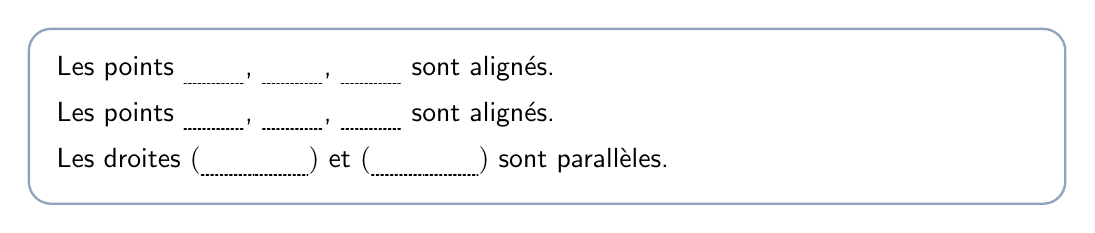
\begin{tikzpicture}
\node[rounded corners=8pt,draw=brandNavy!45,fill=white,line width=0.85pt,text width=12.46cm,inner sep=10.0pt,align=left] {
{\fontsize{9.8}{10.9}\selectfont Les points \LowDotted{0.76}, \LowDotted{0.76}, \LowDotted{0.76} sont alignés.}\par\vspace{0.16cm}
{\fontsize{9.8}{10.9}\selectfont Les points \LowDotted{0.76}, \LowDotted{0.76}, \LowDotted{0.76} sont alignés.}\par\vspace{0.16cm}
{\fontsize{9.8}{10.9}\selectfont Les droites $(\LowDotted{0.66}\LowDotted{0.66})$ et $(\LowDotted{0.66}\LowDotted{0.66})$ sont parallèles.}
};
\end{tikzpicture}

\vspace{0.25cm}
{\bfseries\color{brandNavy}\fontsize{11.2}{12.0}\selectfont Je complète le tableau de proportionnalité}\par\vspace{0.04cm}
\begin{center}
{\renewcommand{\arraystretch}{2.00}\fontsize{10.8}{11.5}\selectfont
$\displaystyle
\begin{array}{|c|c|c|c|}\hline
\textcolor{brandBlue}{\text{Petit triangle}} & \LowDotted{1.18} & \LowDotted{1.18} & \LowDotted{1.18}\\ \hline
\textcolor{brandTeal}{\text{Grand triangle}} & \LowDotted{1.18} & \LowDotted{1.18} & \LowDotted{1.18}\\ \hline
\end{array}$}
\end{center}

\vspace{0.28cm}
{\bfseries\color{brandNavy}\fontsize{11.4}{12.2}\selectfont D'après le théorème de Thalès}\par\vspace{0.06cm}
\begin{center}
$\displaystyle
\frac{\LowDotted{0.92}}{\LowDotted{0.92}}
=
\frac{\LowDotted{0.92}}{\LowDotted{0.92}}
=
\frac{\LowDotted{0.92}}{\LowDotted{0.92}}
$
\end{center}

\vspace{0.27cm}
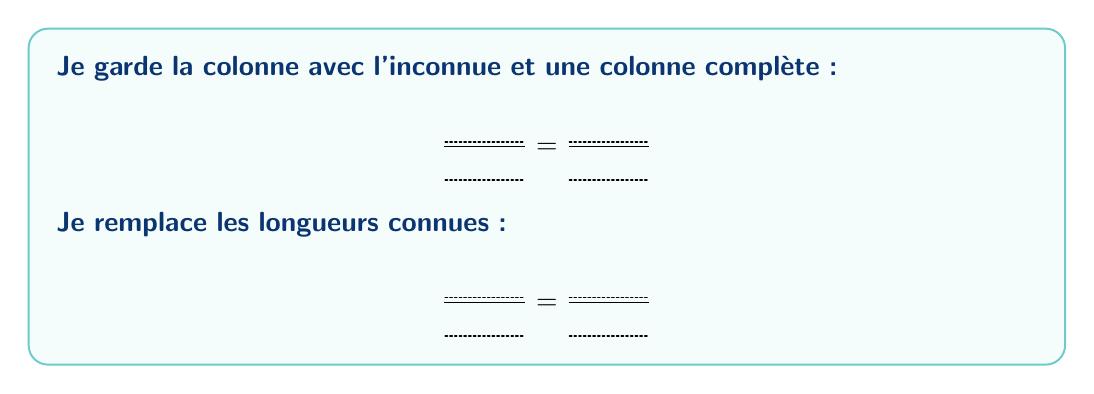
\begin{tikzpicture}
\node[rounded corners=7pt,draw=brandTeal!65,fill=softTeal!30,line width=.70pt,text width=12.46cm,inner sep=10pt,align=left] {
{\bfseries\color{brandNavy} Je garde la colonne avec l'inconnue et une colonne complète :}\par\vspace{0.22cm}
\begin{center}$\displaystyle \frac{\LowDotted{1.00}}{\LowDotted{1.00}}=\frac{\LowDotted{1.00}}{\LowDotted{1.00}}$\end{center}
{\bfseries\color{brandNavy} Je remplace les longueurs connues :}\par\vspace{0.22cm}
\begin{center}$\displaystyle \frac{\LowDotted{1.00}}{\LowDotted{1.00}}=\frac{\LowDotted{1.00}}{\LowDotted{1.00}}$\end{center}
};
\end{tikzpicture}

\vspace{0.22cm}
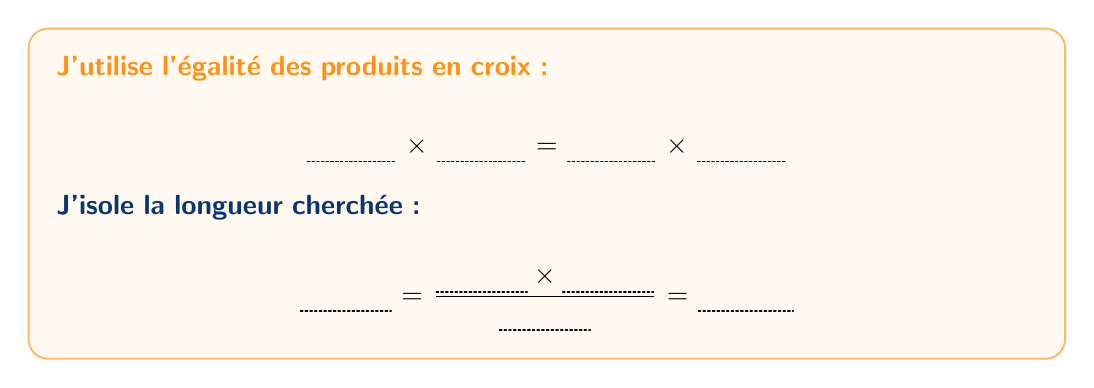
\begin{tikzpicture}
\node[rounded corners=7pt,draw=brandOrange!65,fill=softOrange!35,line width=.70pt,text width=12.46cm,inner sep=10pt,align=left] {
{\bfseries\color{brandOrange} J'utilise l'égalité des produits en croix :}\par\vspace{0.22cm}
\begin{center}\LowDotted{1.12} $\times$ \LowDotted{1.12} $=$ \LowDotted{1.12} $\times$ \LowDotted{1.12}\end{center}
{\bfseries\color{brandNavy} J'isole la longueur cherchée :}\par\vspace{0.22cm}
\begin{center}\LowDotted{1.15} $=$ $\displaystyle\frac{\LowDotted{1.15}\times\LowDotted{1.15}}{\LowDotted{1.15}}$ $=$ \LowDotted{1.20}\end{center}
};
\end{tikzpicture}

\vspace{0.22cm}
\begin{center}
\tikz\node[rounded corners=7pt,draw=brandNavy!55,fill=softBlue!25,line width=.75pt,text width=11.80cm,inner sep=7pt,align=center]{\bfseries\color{brandNavy} Donc \LowDotted{1.20} $=$ \LowDotted{1.35} \LowDotted{0.70}.};
\end{center}
\end{minipage}

\newpage

% ================= PAGE 3 : EXEMPLES =================
\begin{center}
{\fontsize{20.0}{21.0}\selectfont\bfseries\color{brandNavy} Deux exemples entièrement rédigés}\par\vspace{0.02cm}
{\fontsize{11.8}{12.5}\selectfont\bfseries\color{brandTeal} Un cas emboîté et un cas papillon}
\end{center}

\vspace{0.14cm}
{\bfseries\color{brandTeal}\fontsize{12.5}{13.3}\selectfont Exemple 1 — cas emboîté : calculer $MN$}\par\vspace{0.05cm}
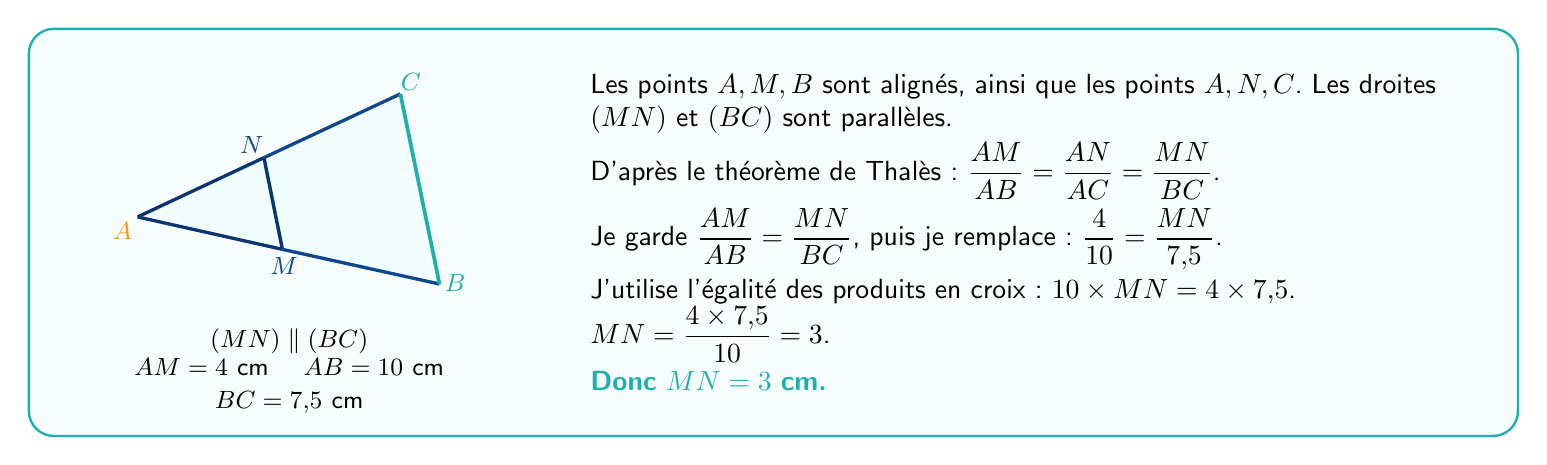
\begin{tikzpicture}
\node[rounded corners=9pt,draw=brandTeal,fill=brandTeal!4,line width=.85pt,text width=18.35cm,inner sep=8pt,align=left] {
\begin{minipage}[c]{6.05cm}
\centering\FigureEmboitee{0.71}\par\vspace{0.08cm}
{\fontsize{9.4}{10.1}\selectfont $(MN)\parallel(BC)$\par $AM=4$ cm \quad $AB=10$ cm\par $BC=7{,}5$ cm}
\end{minipage}\hfill
\begin{minipage}[c]{11.50cm}
Les points $A,M,B$ sont alignés, ainsi que les points $A,N,C$. Les droites $(MN)$ et $(BC)$ sont parallèles.\par\vspace{0.08cm}
D'après le théorème de Thalès :
$\displaystyle \frac{AM}{AB}=\frac{AN}{AC}=\frac{MN}{BC}$.\par\vspace{0.08cm}
Je garde $\displaystyle \frac{AM}{AB}=\frac{MN}{BC}$, puis je remplace :
$\displaystyle \frac{4}{10}=\frac{MN}{7{,}5}$.\par\vspace{0.08cm}
J'utilise l'égalité des produits en croix :
$10\times MN=4\times7{,}5$.\par
$\displaystyle MN=\frac{4\times7{,}5}{10}=3$.\par\vspace{0.08cm}
{\bfseries\color{brandTeal} Donc $MN=3$ cm.}
\end{minipage}
};
\end{tikzpicture}

\vspace{0.36cm}
{\bfseries\color{brandOrange}\fontsize{12.5}{13.3}\selectfont Exemple 2 — cas papillon : calculer $AC$}\par\vspace{0.05cm}
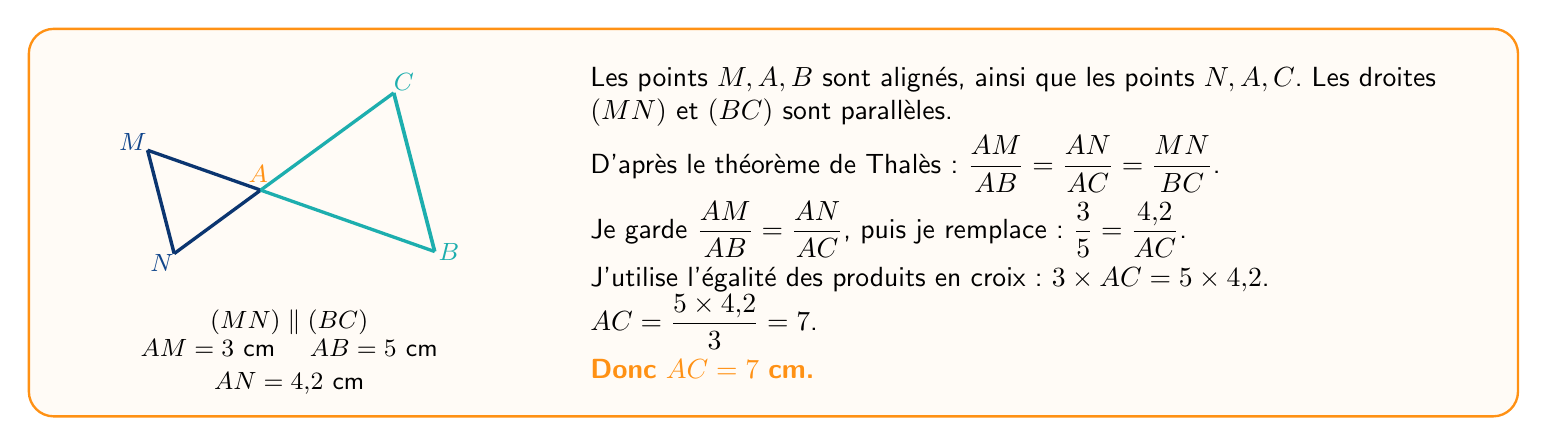
\begin{tikzpicture}
\node[rounded corners=9pt,draw=brandOrange,fill=brandOrange!4,line width=.85pt,text width=18.35cm,inner sep=8pt,align=left] {
\begin{minipage}[c]{6.05cm}
\centering\FigurePapillon{0.65}\par\vspace{0.08cm}
{\fontsize{9.4}{10.1}\selectfont $(MN)\parallel(BC)$\par $AM=3$ cm \quad $AB=5$ cm\par $AN=4{,}2$ cm}
\end{minipage}\hfill
\begin{minipage}[c]{11.50cm}
Les points $M,A,B$ sont alignés, ainsi que les points $N,A,C$. Les droites $(MN)$ et $(BC)$ sont parallèles.\par\vspace{0.08cm}
D'après le théorème de Thalès :
$\displaystyle \frac{AM}{AB}=\frac{AN}{AC}=\frac{MN}{BC}$.\par\vspace{0.08cm}
Je garde $\displaystyle \frac{AM}{AB}=\frac{AN}{AC}$, puis je remplace :
$\displaystyle \frac{3}{5}=\frac{4{,}2}{AC}$.\par\vspace{0.08cm}
J'utilise l'égalité des produits en croix :
$3\times AC=5\times4{,}2$.\par
$\displaystyle AC=\frac{5\times4{,}2}{3}=7$.\par\vspace{0.08cm}
{\bfseries\color{brandOrange} Donc $AC=7$ cm.}
\end{minipage}
};
\end{tikzpicture}

\end{document}
